\section{Face Detection}\label{sec:face-detection}
As I mentioned in the description of pipeline the goal of face detection is to find the location of face within the
image.
This is challenging in unconstrained environments due to various poses, illuminations and occlusions.

To not digress I will describe only system which was put in use during implementation.
The detection algorithm is called MTCNN~\ref{subsec:mtcnn}.

Before going through the process of face detection it is necessary to describe a method called Non-maximum Suppression.

\subsection{Non-maximum Suppression}\label{subsec:nms}
Non-maximum Suppression (NMS) is a filtering algorithm of overlapping bounding
boxes\footnote{\label{foot:bbox}A rectangle describing face position.}.
NMS consists of five simple steps:
\begin{enumerate}
    \item \label{itm:nmss1}Create a list of proposal bounding boxes ordered by confidence score.
    \item Select the bounding box with highest confidence score and add it to the filtered list of boxes.
    \item Compute IoU~\ref{fig:iou} between the selected bounding box and all the remaining ones.
    \item Remove all the boxes whose IoU is higher than some predetermined threshold.
    \item Go to~\ref{itm:nmss1} and repeat the process until there are no remaining bounding boxes within the original list.
\end{enumerate}

Having NMS defined we can proceed with actual face detection.

\subsection{MTCNN}\label{subsec:mtcnn}
MTCNN~\cite{MTCNN} stands for Multi-task Cascaded Convolutional Networks.
This model consists of three stages.

\subsubsection{Stage 1}
The first stage is called \textbf{Proposal Network} (P-Net) and its role is to find the candidate windows and their
bounding box regression vectors.
P-Net is fully convolutional neural network.

Before passing the image to P-Net image pyramid is created.
In other words the original image is resized to many different sizes.
This gives the model scale invariance.

At this point we feed the images to the net.

The net produces many bounding boxes with varying confidence.
We parse the output and delete the boxes with low confidence score.

Now we standardize the coordinate system by converting the boxes from resized image to that of unscaled one.

First we run NMS~\ref{subsec:nms} once for every scaled image.
Then we put all the survivors into one list and run NMS once more.

Before passing the boxes to stage 2 we make the boxes square by elongating the shorter sides.

\subsubsection{Stage 2}
Candidates from P-Net are fed to another CNN,
The objective of this net is to filter out a large number of false positives, to perform calibration with bounding
box regression and to merge
This stage is called \textbf{Refined Network} (R-Net).

\begin{figure}[H]
    \centering
    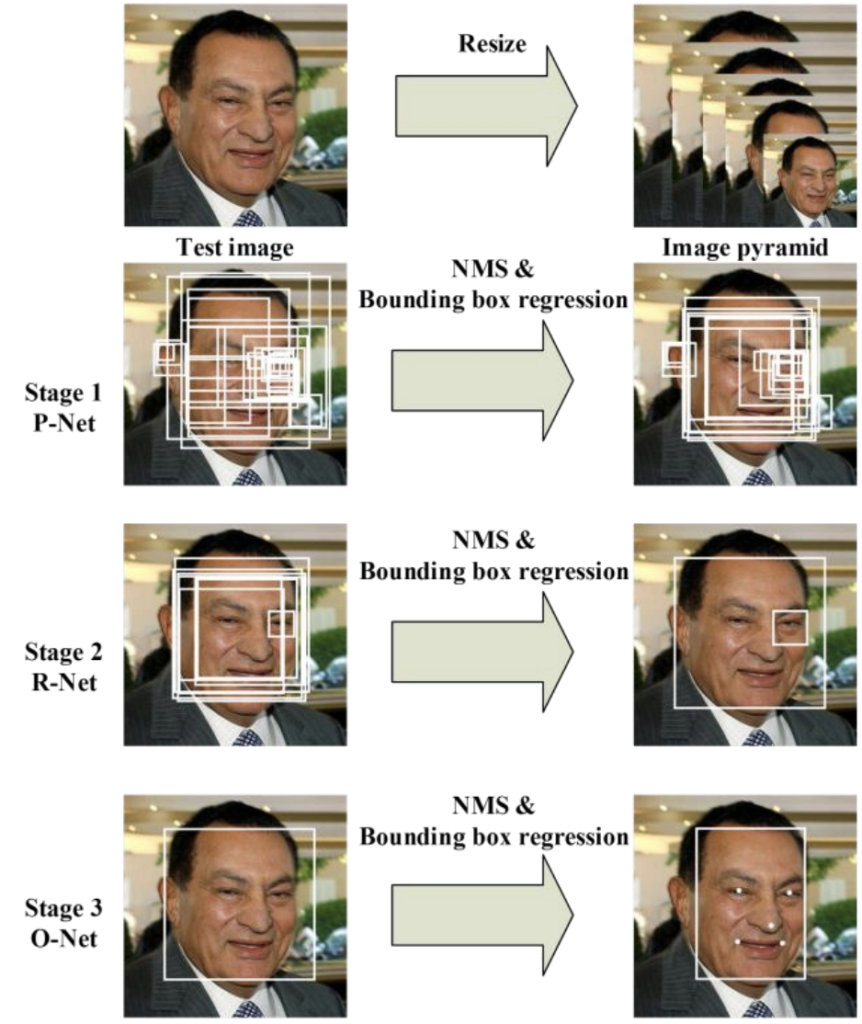
\includegraphics[width=0.8\columnwidth]{images/face-recognition/mtcnn.png}
    \caption{MTCNN face detection pipeline~\cite{MTCNN}.}
    \label{fig:mtcnn}
\end{figure}